\section{Methodology}

Below, some detailed instruction regarding the typsetting can be found. These instructions are based on the official AIAA template and follow the guidelines of AE2223-I.

\subsection{Document Text}
The default font for your report is Times New Roman, 11-point size. The first line of every paragraph should be indented, with the exception of paragraphs that follow a heading or a blank line (in case of the latter, use \verb+\noindent+). All lines should be single-spaced. Default margins are 1” on all sides. In the electronic version of this template, all margins and other formatting is preset. Limit the use of abbreviations such as e.g. or viz.

\subsection{Headings}
The title of your paper should be typed in bold, 18-point type, with capital and lower-case letters, and centered at the top of the page. The names of the authors and the affiliation should follow on separate lines below the title. Author names are centered, and affiliations are centered and in italic type.

\begin{itemize}
    \item Major headings (\verb+\sections{}+) are bold 11-point font, centered, and numbered with Roman numerals.
    \item Subheadings (\verb+\subsections{}+) are bold, flush left, and numbered with capital letters.
    \item Sub-subheadings (\verb+\subsubsections{}+) are italic, flush left, and numbered (1. 2. 3. etc.)
\end{itemize}

\subsection{In-text References}
Choose and output style that you will use for your references and apply this style consistently throughout your paper. Make sure that you know what your in text references should look like and how different publication types (e.g. books, journal papers etc.) should  be formatted in the reference list.  Examples of references styles are:

\begin{itemize}
    \item AIAA, in which the references are numbered following the order of appearance in your text (for examples of titles in the Reference list, see the “References” section on page 4 of this template. For documentation, see article.bib), and
    \item APA, in which you present the name(s) of the author(s) and the year of publication in your text and references are sorted alphabetically in the reference list.
\end{itemize}

\subsection{Footnotes}
Footnotes, where they appear, should be placed above the 1” margin at the bottom of the page. To insert footnotes into the template, use \verb+\footnote{}+. Superscript numbers for footnotes are used by default. Use footnotes scarcely and only to provide additional information that is not essential to understand your argumentation in the main text.

\subsection{Images, Figures, and Tables}
Captions are bold and justified, with a period and a single tab (no hyphen or other character) between the figure number and figure description.

Place figure captions below all figures; place table titles over the tables. If your figure has multiple parts, include the labels “a),” “b),” etc. below and to the left of each part, above the figure caption. Please verify that the figures and tables you mention in the text actually exist. When citing a figure in the text, use the abbreviation “Fig.” except at the beginning of a sentence. Do not abbreviate “Table.” Number each different type of illustration (i.e., figures, tables) sequentially with relation to other illustrations of the same type.

Figure axis labels are often a source of confusion. Use words rather than symbols. As in the example below (\cref{fig:sample}), write the quantity “Magnetization” rather than just “M.” Do not label axes with units only.
Figure labels must be legible, approximately 8-12 point type. Only use colors for your illustrations if needed.

\begin{figure}[htb]
    \centering
    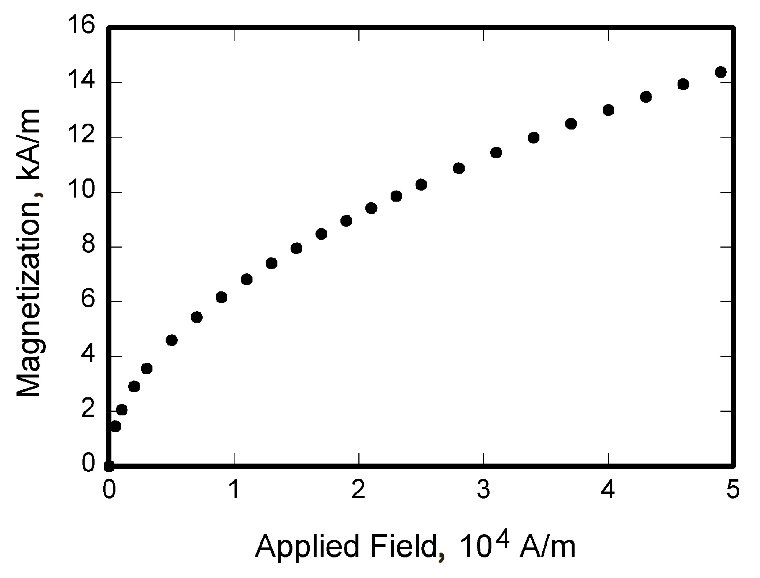
\includegraphics[width=0.4\linewidth]{figures/graph.jpg}
    \caption{Magnetization as a function of applied field}
    \label{fig:sample}
\end{figure}

\subsection{Equations, Numbers, Symbols, and Abbreviations}
Equations are centered and numbered consecutively, with equation numbers in parentheses flush right, as in \cref{eqn:sample}. Insert a blank line on either side of the equation.
\begin{equation}
    \label{eqn:sample}
    L = C_L \frac{1}{2}\rho V^2 S
\end{equation}

\noindent Be sure that the symbols in your equation are defined before the equation appears, or immediately following. Italicize symbols (T might refer to temperature, but T is the unit tesla). Refer to “Eq. (1),” not “(1)” or “equation (1)” except at the beginning of a sentence: “Equation (1) is…”

Define abbreviations and acronyms the first time they are used in the text, even after they have already been defined in the abstract. Do not use abbreviations in the title.
